\documentclass[border=4pt]{standalone}
\usepackage{tikz}
\usetikzlibrary{arrows,positioning}
\begin{document}
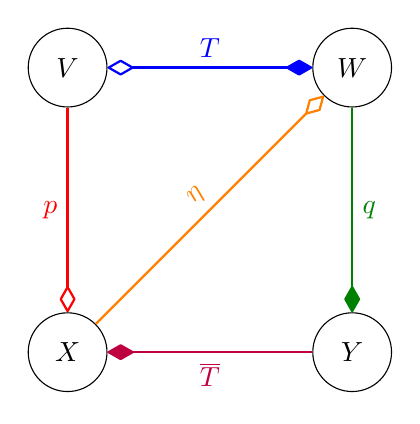
\begin{tikzpicture}[
  node distance=2.6cm,
  object/.style={draw,circle,minimum size=10mm,inner sep=1pt}
]
  \node[object] (V) {$V$};
  \node[object,right=of V] (W) {$W$};
  \node[object,below=of V] (X) {$X$};
  \node[object,right=of X] (Y) {$Y$};

  \draw[blue,line width=.8pt,{open diamond}-{diamond}] (V) -- node[above] {$T$} (W);
  \draw[red,line width=.8pt,-{open diamond}] (V) -- node[left] {$p$} (X);
  \draw[green!50!black,line width=.8pt,-diamond] (W) -- node[right] {$q$} (Y);
  \draw[purple,line width=.8pt,{diamond}-] (X) -- node[below] {$\overline{T}$} (Y);
  \draw[orange,line width=.8pt,-{open diamond}] (X) -- node[above,sloped] {$\eta$} (W);
\end{tikzpicture}
\end{document}
